% ======================= 1. INTRODUCCIÓN =======================
\section{Introducción y justificación}\label{sec:intro}

El SIMA es la red de monitoreo de la calidad del aire del Gobierno de Nuevo León. Opera desde 1992 y sus 15 estaciones automáticas en la ZMM miden cada hora contaminantes criterio y variables meteorológicas. Con esos datos calcula el Índice Aire y Salud, elabora pronósticos y activa el programa de respuesta a contingencias (Sistema Integral de Monitoreo Ambiental [SIMA], 2026). El Plan Integral de Gestión Estratégica de la Calidad del Aire 2023–2033 (PIGECA) le asigna generar información confiable para evaluar la calidad del aire y sus impactos, y contempla medidas de fortalecimiento de la red y de pronóstico (Secretaría de Medio Ambiente del Estado de Nuevo León [SMA] y Clean Air Institute [CAI], 2024).

El PM2.5 es el contaminante en el que nos enfocamos. Un metaanálisis de 196 artículos asoció la exposición de corto plazo a partículas con mayor mortalidad total, cardiovascular y respiratoria (Orellano et al., 2020), y la Organización Mundial de la Salud fijó en 2021 una guía de 15\ugm{} para el promedio de 24\,h (World Health Organization [WHO], 2021). Usamos como umbral 25\ugm, el límite de 24\,h de la NOM-025-SSA1-2021 en su quinto año de aplicación (Secretaría de Salud, 2021). Es una \textbf{referencia fija para comparar todo el periodo, no una evaluación del cumplimiento normativo}, porque los límites aplicables cambiaron entre 2021 y 2025. El resultado describe concentraciones, no riesgo individual: por debajo de 25\ugm{} el riesgo no es nulo.

\textbf{Antecedentes en la ZMM.} Aguirre-López et al. (2022) describieron en siete estaciones una tendencia decreciente del PM10 con ciclo anual (2010–2018) y propusieron incorporar la meteorología. Hernández-Romero et al. (2026) documentaron la persistencia de excedencias de PM10, PM2.5 y O\textsubscript{3}, con máximos de partículas en la temporada seca-fría. Martínez-Cinco et al. (2016) atribuyeron el PM2.5 otoñal sobre todo a emisiones vehiculares que se acumulan con viento débil. Ramírez-Velarde et al. (2024) combinaron componentes principales y clasificadores con meteorología del SIMA para anticipar contingencias. Fuera de México, Vélez-Pereira et al. (2025) clasificaron con regresión logística las superaciones diarias de PM2.5 y PM10 en varias ciudades de Chile, como base simple para alertas tempranas.

\textbf{Justificación para SIMA.} Saber en qué temporadas y con qué condiciones la meteorología del día añade información sobre los días de PM2.5 alto es un paso previo a una alerta con pronóstico, que el área de pronósticos de SIMA dijo que le interesa (SIMA, comunicación personal, 15 de octubre de 2026). Primero hay que medir cuánto ayuda la meteorología observada; si no ayuda con datos medidos, tampoco ayudará con datos pronosticados.

\textbf{Alcance dentro del reto.} El proyecto cubre cuatro puntos del reto: la clasificación de días con y sin superación del umbral fijo de 25\ugm, los factores meteorológicos asociados, la distribución por estación y el contexto de fuentes de las estaciones más afectadas. No evalúa el cumplimiento normativo ni el efecto de la política ambiental antes y después de 2022 o de la pandemia (Schiavo et al., 2023); estos últimos quedan como preguntas nuevas (Sección~\ref{sec:conclusiones}).

% ======================= 2. PROBLEMÁTICA =======================
\section{Problemática y objetivo}\label{sec:objetivo}

\textbf{Pregunta.} ¿En qué medida la meteorología del día mejora la clasificación retrospectiva de los días-estación con PM2.5 promedio de 24\,h superior a 25\ugm, respecto de un modelo que solo considera la estación de monitoreo y la temporada, en 13 estaciones de la ZMM durante 2021–2025?

\textbf{Objetivo general.} Cuantificar, con validación temporal, la mejora en el área bajo la curva ROC (\dauc) que aporta la meteorología del día (M1) sobre un modelo con estación y temporada (M0), con análisis discriminante lineal (LDA), la técnica fijada en el protocolo, y con regresión logística en paralelo.

\textbf{Objetivos específicos.} (1) Construir una base día-estación con limpieza documentada e imputación validada, sin imputar la respuesta. (2) Describir la estructura de correlación de la meteorología con componentes principales (PCA). (3) Estimar M0 y M1 y su diferencia, con intervalos que respeten la dependencia temporal y espacial. (4) Identificar en qué temporadas y con qué variables se concentra la mejora, y qué permiten concluir los dos clasificadores. (5) Traducir los resultados en recomendaciones para SIMA.

\textbf{Unidad, respuesta y temporadas.} La unidad de análisis es el \emph{día-estación}: el promedio de 24\,h de una estación en un día. La respuesta \texttt{supera\_25} vale 1 si ese promedio, calculado con al menos 18 horas observadas de PM2.5, supera 25\ugm. Las \textbf{temporadas} son tres periodos operativos fijados en la etapa 1, antes de modelar: \textbf{seca-fría} (noviembre a febrero), \textbf{seca-cálida} (marzo a mayo, la primavera seca y caliente previa a las lluvias) y \textbf{cálida-húmeda o de lluvias} (junio a octubre). Separan bien el riesgo: en la base final la superación es de 38\,\%, 36\,\% y 13\,\%, respectivamente (Tabla~\ref{tbl:b-exclusiones}).

\textbf{Evolución del alcance.} En la etapa 1 propusimos identificar regímenes multicontaminante con conglomerados. La retroalimentación pidió acotar el problema y lo reenfocamos en el PM2.5 y en la comparación M0–M1 (etapa 2). En la etapa 4 atendimos la retroalimentación sobre la imputación y sobre el uso del LDA. \textbf{Alcance:} clasificación retrospectiva con meteorología observada del mismo día, no pronóstico.

% ======================= 3. ÁREA DE ESTUDIO =======================
\section{Área de estudio: estaciones y factores geográficos}\label{sec:area}

La ZMM ocupa un valle rodeado por la Sierra Madre Oriental al sur y al oeste y por sierras como el Cerro de la Silla. Las 13 estaciones de la muestra van de 334\,m (SE3, Cadereyta) a 702\,m de altitud (NO2, García); el oeste (Santa Catarina, San Pedro y García) es más alto y encajonado (Figura~\ref{fig:mapa}; nombres, municipios y días por estación en la Tabla~\ref{tbl:estaciones}, Anexo~B). En nuestros datos domina el flujo del este: la componente zonal del viento es negativa (\emph{u} < 0) en el 80\,\% a 98\,\% de los días en 11 de las 13 estaciones, con dirección resultante entre 68° y 140° (del este al sureste). Las excepciones son NE2 (62\,\%) y SO2 (68\,\%). Según SIMA, el viento predominante sale del área metropolitana por Santa Catarina y García (comunicación personal, 15 de octubre de 2026).

\begin{figure}[!htbp]
\centering
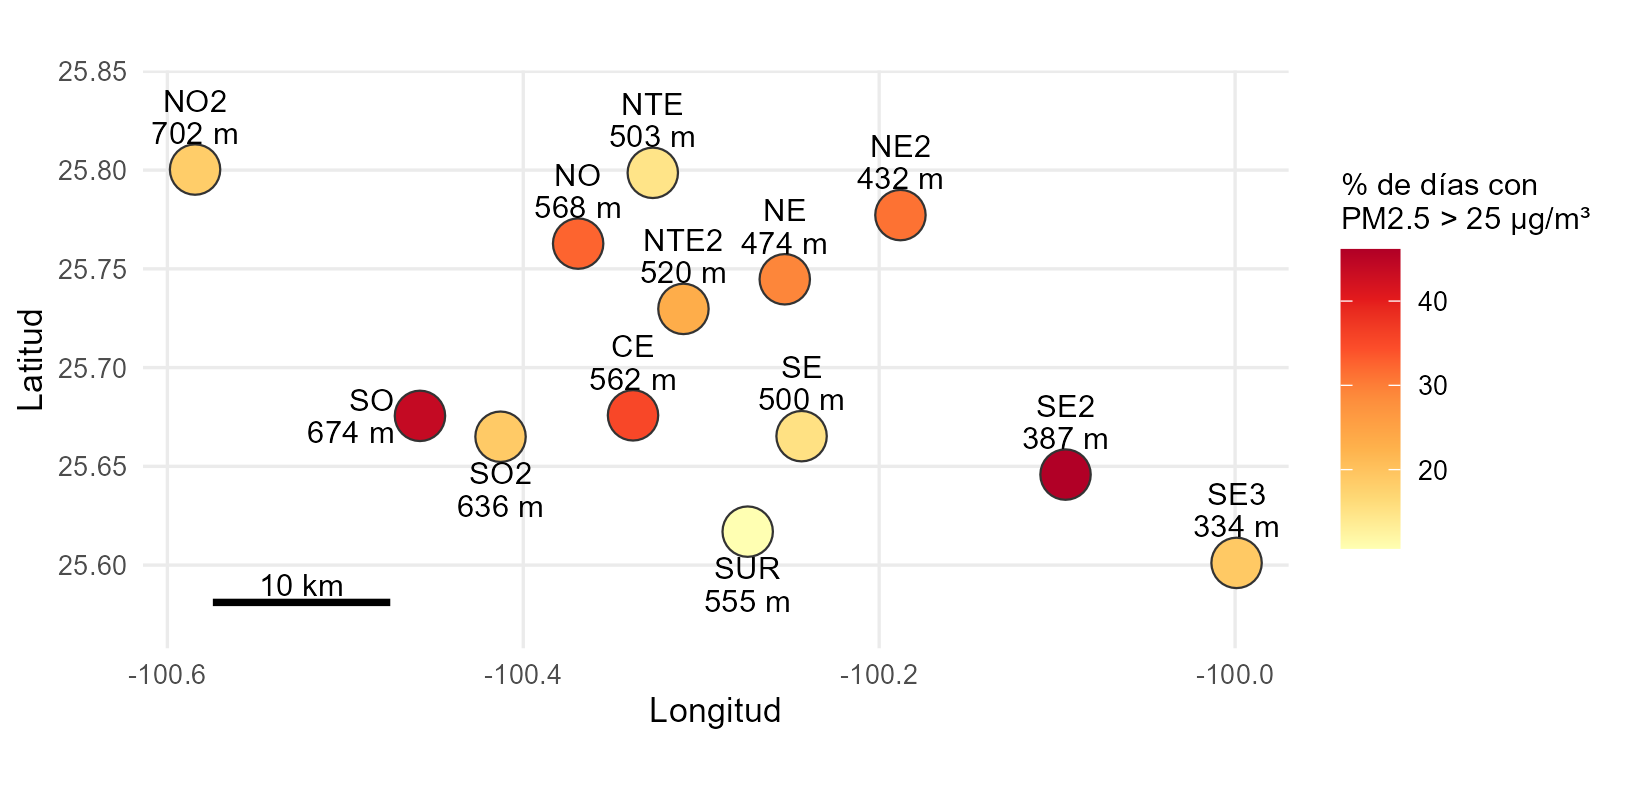
\includegraphics[width=0.70\textwidth]{figuras/mapa_estaciones_informe.png}
\caption{Estaciones de la muestra, con su altitud (m s.\,n.\,m.) y el porcentaje de días-estación con PM2.5 > 25\ugm{} en el análisis final (base v2, 2021–2025, n = 17\,828). Solo coordenadas, sin mapa base. El porcentaje de NO2 incluye el periodo con PM2.5 anómalo (Anexo~C). Elaboración propia con datos de SIMA.}
\label{fig:mapa}
\end{figure}

La Figura~\ref{fig:mapa} muestra que la superación no sigue la altitud: SO (674\,m) y SE2 (387\,m) tienen los porcentajes más altos y están en extremos opuestos del valle, mientras que SE3 (334\,m), la más baja, está por debajo de la mitad de la red. El porcentaje bajo de NO2 no sirve para este argumento: en buena parte refleja un problema de su equipo de PM2.5 (Tabla~\ref{tbl:b-cambios}).



\textbf{Contexto por estación.} SIMA describió las fuentes de las dos estaciones con más superaciones (comunicación personal, 15 de octubre de 2026), y las contrastamos con nuestros datos:
\begin{itemize}
\item \textbf{SE2 (Juárez).} Es el primer receptor de la pluma de la refinería: por la altura de los quemadores, la dispersión pasa por encima de Cadereyta (SE3) y llega a Juárez. Además, hay crecimiento urbano, vialidades sucias con resuspensión, quemas nocturnas, transporte pesado y obras viales. En nuestros datos, SE2 tiene el viento más débil de la red (1.55\,m/s de media) y el PM2.5 más ligado al PM10 (Spearman 0.82). Su cociente PM2.5/PM10 (mediana 0.40) está entre los más altos de la red (0.25 a 0.42): la fracción gruesa sigue siendo la mayor parte, pero la fina pesa relativamente más que en otras estaciones y sube en los días con superación (0.46 frente a 0.35). De forma descriptiva, en enero el PM2.5 medio de SE2 subió de 33.1 a 43.1\ugm{} entre 2023 y 2024 (19 y 30 días con dato), mientras que en SE3 no cambió (22.4\ugm); va en la misma dirección que el alza que el gobierno estatal atribuyó a la refinería, aunque sus cifras no son las nuestras (Gobierno del Estado de Nuevo León, 2024).
\item \textbf{SO (Santa Catarina).} Es una zona industrial de entrada, con suelo semidesértico, carga vehicular y receptora de la salida del viento. En nuestros datos los días con superación tienen viento más débil (diferencia de medias estandarizada de la rapidez −0.76, la mayor de la red) y un flujo del este menos intenso (\emph{u} de −1.16 frente a −2.01\,m/s). Con promedios diarios no se puede separar la acumulación local del transporte desde la ciudad.
\item \textbf{SUR (Pueblo Serena).} Su reubicación se ve en los datos: pasó de 3.0\,\% de días con superación en 2021 a 10–12\,\% desde 2022, y su presión frente a la red cambió +5.7\,mm\,Hg en la fecha de reubicación.
\end{itemize}
Son explicaciones de contexto, consistentes con los datos, que no se pueden atribuir sin inventarios de emisiones ni análisis horario de transporte.

\textbf{Cambios en la red (Tabla~\ref{tbl:b-cambios}, Anexo~B).} El PIGECA registra reubicaciones de NO (junio de 2021), SE, SO, NTE y SUR (septiembre de 2021) y NE (febrero de 2022) (SMA y CAI, 2024, p.~91); el entrenamiento excluye los días previos (D23). Los sensores de viento se renovaron en 2021 (por eso se excluye 2020) y cinco equipos de PM2.5 cambiaron en 2025. El PM2.5 de NO2 baja a la mitad del nivel de la red con su PM10 normal, y la radiación de NO2 y NTE es muy baja. Las sensibilidades a estos cambios dan mejoras de 0.079 a 0.082 (Tabla~\ref{tbl:robustez}, Anexo~C).

% ======================= 4. PREPARACIÓN =======================
\section{Preparación de la base de datos}\label{sec:preparacion}

\subsection{Datos y diagnóstico}\label{sec:datos}
SIMA entregó seis libros de Excel (2020–2025) con 87 hojas estación-año y datos horarios de 15 estaciones y 15 variables. Sobre los valores horarios esperados faltaba el 12.3\,\%. \textbf{En el PM2.5 faltaba el 26.0\,\% de las horas} (17.2\,\% en las 13 estaciones de la muestra, 2021–2025), y de esas horas el 44\,\% está en huecos de más de una semana. Los faltantes son sobre todo apagones largos: en las seis variables que se imputan o se modelan, entre el 51\,\% y el 82\,\% de las horas faltantes están en huecos de más de un día (Tabla~\ref{tbl:b-huecos}, Anexo~B). Esto descarta reconstruir esos huecos con métodos locales y motiva imputar a nivel diario con información de la red (Sección~\ref{sec:imputacion}).

\subsection{Limpieza por reglas}
Cada hora de cada variable conserva una bandera que indica si es válida o por qué se anuló; no se elimina ninguna fila (Tabla~\ref{tbl:b-limpieza}, Anexo~B). Las reglas de consistencia espacial (D14) comparan cada lectura con la mediana de la red a la misma hora (Fiebrich et al., 2010). La regla D15 anula la radiación de todo un día si su media de madrugada supera 0.02\,kW/m², y el viento que excede por mucho al de la red (Estévez et al., 2011); se agregó porque la exploración encontró radiación nocturna en NO2, SE3 y CE y vientos imposibles en SO2 y NE2. En total se invalidó el 0.7\,\% de los valores. Los extremos que pasan todas las reglas se conservan, porque pueden ser concentraciones reales. Excluimos 2020 del modelado, porque el viento cambió de nivel con la renovación de sensores de 2021 y por el confinamiento, y las estaciones NE3 y NO3, que casi no miden PM2.5. El detalle de cada regla está en el Anexo~B.

\subsection{Imputación}\label{sec:imputacion}
\textbf{Principio: la respuesta no se imputa (D18).} El PM2.5 diario se calcula solo con al menos 18 horas observadas, el criterio de suficiencia de la NOM-025-SSA1-2021. Imputar el PM2.5 crearía etiquetas de superación que nadie midió, y atiende la advertencia de SIMA sobre los huecos largos en Juárez y Santa Catarina. El costo es perder 526 días-estación con respuesta válida frente a la etapa 3. Las ventanas grandes de la meteorología se recuperan a nivel diario con la información de la red (D20); las del PM2.5 no se rellenan.



\textbf{Imputación horaria de la meteorología (D19).} Usamos los métodos de la fuente principal del curso, el paquete imputeTS (Moritz \& Bartz-Beielstein, 2017): interpolación lineal, spline y de Stineman, media móvil exponencial, filtro de Kalman, descomposición estacional y LOCF como piso. Los elegimos por enmascaramiento solo en 2021–2023: en tramos completos borramos bloques de 1 a 24\,h que sí conocemos, los imputamos con cada método y medimos el error del \textbf{promedio diario}, que es lo que entra al modelo. La regla, fijada antes de ver los resultados y corregida antes de cerrar las decisiones (registro de cambios de la fase A), descalifica los métodos cuyas imputaciones revierte la revalidación en más de 5\,\%. Exige además un error diario de a lo más el 10\,\% de la desviación de la anomalía de cada variable. La Tabla~\ref{tbl:imputacion} (Anexo~B) resume el método elegido por variable, y la Figura~\ref{fig:imputacion} (Anexo~B) muestra que en huecos de 6 a 24\,h la descomposición estacional comete cerca de la mitad del error de la interpolación lineal y que, en el PM2.5, la interpolación aplana los picos, otra razón para no imputar la respuesta. No usamos imputación por vecinos cercanos (KNN).

\textbf{Imputación diaria de la meteorología (D20).} Con la imputación horaria quedan días con una a cuatro de las ocho variables faltantes, sobre todo radiación y humedad. Para recuperarlos comparamos tres métodos en una validación por enmascaramiento con el patrón real de faltantes de 2021–2023. El primero es la mediana de las otras estaciones ese día, ajustada por la diferencia media de la estación, un método de efecto por sitio en la línea de Plaia y Bondì (2006). Los otros dos son MICE con \emph{predictive mean matching} (van Buuren \& Groothuis-Oudshoorn, 2011) y la media de estación × temporada. \textbf{En error puntual, la mediana ajustada y MICE quedan casi empatadas:} RMSE relativo medio de 0.450 frente a 0.436 si se promedian las cinco imputaciones de MICE; la mediana gana en seis de las ocho variables, incluidas temperatura y humedad, las que más faltan en 2024–2025, y MICE gana en lluvia y radiación. Una sola base de MICE tiene más error (0.593), pero eso es esperable, porque el \emph{predictive mean matching} agrega variabilidad a propósito; la media de estación × temporada queda en 0.736. Elegimos la mediana ajustada por ser determinista y simple, y usamos MICE como sensibilidad del clasificador, con 20 bases imputadas: \dauc{} = 0.078 (Tabla~\ref{tbl:robustez}). Ninguna imputación usa el PM2.5 ni la superación como predictor. Moons et al. (2006) muestran que incluir la respuesta al imputar predictores puede reducir el sesgo de las asociaciones; aquí se excluyó para conservar una evaluación predictiva en la que la respuesta de prueba no interviene en los predictores. La idea de aprovechar la red coincide con antecedentes que encontraron mejores imputaciones con información de estaciones vecinas (Quinteros et al., 2019; Belachsen \& Broday, 2022) y suficiencia de métodos simples para promedios diarios (Hadeed et al., 2020).

\textbf{Imputación de referencia del curso.} El curso recomienda como referencia de imputación con datos del SIMA el trabajo MIMA-v1 (Gómez et al., 2025; Gómez Santos et al., 2027), un modelo generativo (SAITS + CSDI) que reconstruye series horarias completas, incluidos los huecos largos. \textbf{No lo usamos porque solicitamos su dataset imputado y no obtuvimos acceso a tiempo.} El análisis natural habría sido una sensibilidad con su meteorología imputada en sus 9 estaciones (enero de 2021 a junio de 2025), conservando nuestro PM2.5 observado como respuesta, lo que es compatible con no imputar la respuesta (D18). Ese análisis tendría dos límites de alcance: su cobertura no incluye Juárez (SE2), Cadereyta (SE3), SUR ni NE2, y su PM2.5 imputado no se usaría como etiqueta. Hay coincidencias con su trabajo: en su comparación de métodos clásicos, la interpolación lineal tuvo el menor error (MAE de 4.01) y la descartaron porque suaviza los picos. Nuestro enmascaramiento confirma ese suavizado en el PM2.5; por eso no imputamos la respuesta y elegimos el método horario de la meteorología con validación. De las fuentes del curso tomamos los métodos de imputeTS (Moritz \& Bartz-Beielstein, 2017) y la validación por enmascaramiento.

\subsection{Transformaciones}
\begin{itemize}
\item \textbf{Agregado diario:} un valor diario existe con al menos 18 horas válidas de esa variable.
\item \textbf{Viento:} componentes \emph{u} (este-oeste) y \emph{v} (norte-sur) y rapidez, porque la dirección es circular.
\item \textbf{Lluvia:} horas con lluvia en el día, porque la unidad de la cantidad no está confirmada.
\item \textbf{Presión:} anomalía respecto de la media de su sitio en el entrenamiento (D17); separa la altitud (medias de 700.8 a 731.5\,mm\,Hg) del efecto meteorológico.
\item \textbf{Escalado:} todas las variables se estandarizan con medias y desviaciones del entrenamiento.
\item \textbf{Sin logaritmos (D16):} en la validación progresiva, transformar la lluvia y el viento solo subió el AUC 0.003 y 0.007, y el logaritmo sobrecorregía la asimetría del viento (de +0.37 a −0.98).
\end{itemize}

\subsection{Muestra final, exclusiones y posible sesgo}\label{sec:muestra}
La Tabla~\ref{tbl:exclusiones} clasifica los 23\,738 días-estación posibles (13 estaciones × 1\,826 días) según su causa de exclusión: la imputación diaria recupera los días con una a cuatro meteorológicas faltantes, no los que tienen cinco o más, y el entrenamiento excluye los días previos a cada reubicación (D23), porque corresponden a otro sitio. El análisis final queda con \textbf{17\,828 días-estación}: 10\,965 de entrenamiento (2021–2023; 25.9\,\% de superación) y 6\,863 de prueba (2024–2025; 26.2\,\%). Frente a la etapa 3 hay 2\,438 días más, sobre todo en García (NO2: de 511 a 1\,532), donde faltaba la radiación, y en Escobedo (NTE: de 597 a 1\,373), donde faltaba la humedad (Anexo~C). En la prueba, el 27\,\% de los días (1\,876 de 6\,863) tiene al menos una variable meteorológica completada con la mediana de la red, sobre todo en NTE (646 de 662) y NE (452 de 657). No es una fuga de información, porque la imputación no usa la respuesta, pero conviene tenerlo presente: sin imputación diaria la mejora es de 0.071 (Tabla~\ref{tbl:faltantes}).

\begin{table}[!htbp]
\centering\small
\caption{Causas de exclusión de los 23\,738 días-estación posibles (2021–2025) y respuesta de cada grupo donde existe. Las causas (a) a (d) suman el total; (e) es parte de (b) y (c). Detalle por estación, temporada y año en el Anexo~B.}
\label{tbl:exclusiones}
\begin{tabularx}{\textwidth}{Lrrcrrr}
\toprule
Grupo & Días-estación & \% & ¿En el análisis? & \% superación & Mediana de PM2.5 & \% con PM2.5 > 40\\
\midrule
(a) Sin PM2.5 suficiente (< 18\,h observadas) & 4\,346 & 18.3 & No & — & — & —\\
(b) Respuesta y meteorología completa & 15\,011 & 63.2 & Sí & 27.0 & 18.5 & 5.5\\
(c) Respuesta y 1–4 meteorológicas imputadas & 4\,192 & 17.7 & Sí & 23.5 & 17.7 & 3.7\\
(d) Respuesta y 5–8 meteorológicas faltantes & 189 & 0.8 & No & 33.3 & 18.7 & 5.8\\
(e) De (b) o (c), previos a una reubicación & 1\,375 & 5.8 & No & 29.5 & 19.2 & 4.3\\
\bottomrule
\end{tabularx}
\end{table}

Donde hay respuesta, los excluidos se parecen a los incluidos: 33.3\,\% de superación en (d), con solo 189 días, y 29.5\,\% en (e), frente a 27.0\,\% en (b). Los días que recupera la imputación (c) tienen menos superación en promedio (23.5\,\%), pero la diferencia cambia de signo según la estación: en NO2, donde faltaba la radiación, es de 22.7\,\% en (c) y 9.8\,\% en (b). Con casos completos, la etapa 3 daba a NO2 10.0\,\% de superación y la base final 18.4\,\%: esa exclusión sesgaba la muestra. Los días sin PM2.5 suficiente (a) se concentran en NO (57\,\% de sus días, con un hueco de 532 días desde marzo de 2024), NE2 (33\,\%) y SUR (26\,\%), y en 2024–2025 (24\,\% y 30\,\%, frente a 10–15\,\% antes); la mitad están en huecos de más de una semana y se reparten casi igual entre temporadas. Su PM10, disponible en el 86\,\% de ellos, es menor que el de los días con respuesta en 31 de 39 combinaciones de estación y temporada, así que no parecen concentrarse en días de contaminación alta. Aun así, no podemos descartar un sesgo por datos faltantes, sobre todo en la prueba y en NO y NE2. La Tabla~\ref{tbl:faltantes} resume qué se imputó, qué se excluyó y qué mostraron las sensibilidades.

\begin{table}[!htbp]
\centering\small
\caption{Resumen del tratamiento de los datos faltantes: qué se imputó, qué se excluyó y qué mostró el análisis de sensibilidad (\dauc{} de M1 frente a M0 con LDA en la prueba; análisis final: 0.079 [0.054, 0.104]).}
\label{tbl:faltantes}
\begin{tabularx}{\textwidth}{>{\raggedright\arraybackslash}p{2.1cm}LL}
\toprule
Tratamiento & Qué datos & Sensibilidad (\dauc{} [IC 95\,\%])\\
\midrule
Se imputó & Meteorología horaria en huecos cortos (2 a 12\,h según la variable; Tabla~\ref{tbl:imputacion}, Anexo~B) y meteorología diaria de los días con 1–4 de 8 variables faltantes (4\,192 días-estación) & Sin imputación diaria (casos completos): 0.071 [0.047, 0.096]; con MICE (m = 20): 0.078 [0.055, 0.103]; imputación diaria solo con ≤ 2 faltantes: 0.077 [0.052, 0.102]\\
No se imputó & PM2.5 (la respuesta): solo se usa con ≥ 18\,h observadas & PM2.5 interpolado en huecos ≤ 3\,h: 0.079 [0.053, 0.105]\\
Se excluyó & (a) días sin PM2.5 suficiente (4\,346), (d) días con 5–8 meteorológicas faltantes (189) y (e) días previos a una reubicación (1\,375, solo en el entrenamiento) & Reubicaciones según SIMA: 0.081 [0.054, 0.107]; los excluidos con respuesta tienen una superación parecida a los incluidos (Tabla~\ref{tbl:exclusiones})\\
\bottomrule
\end{tabularx}
\end{table}
